% Chapter 1

\chapter{Introduction} % Main chapter title

\label{Chapter1} % For referencing the chapter elsewhere, use \ref{Chapter1} 

%----------------------------------------------------------------------------------------

% Define some commands to keep the formatting separated from the content 


%----------------------------------------------------------------------------------------

\section{In the Beginning}
What is planning? It can be defined as follows: "Explicit deliberation process that chooses and organises actions by anticipating their outcomes" \cite{PlanningBook}; in other words, from a predefined initial state we predict the set of actions used to achieve a predefined goal state. There are many ways we can do this for different scenarios within the domain of planning, but this thesis will concentrate on classical planning, which is a subset of the planning domain. 

So, what is classical planning? "It refers generically to planning for restricted state-transition systems" \cite{PlanningBook}. This is the oldest type of planning and is also known as STRIPS programming (Stanford Research Institute Problem Solver). STRIPS was a planner developed at Stanford University in 1971 \cite{Strips} and its goal was to find a sequence of actions that could prove a goal formula true.

We can class planners in the domain of 'State Transition Systems'. In the example at Figure \ref{fig:StateTransition} we have multiple blocks and a robot. The robot can move from one location to anther as well as pick up and put down the blocks from one location to another. Each picture is a set of states and the arrows represent each new state. We say each state transition is deterministic, meaning that it leads to just one other state. 
\begin{figure}[!htb]
    \centering
    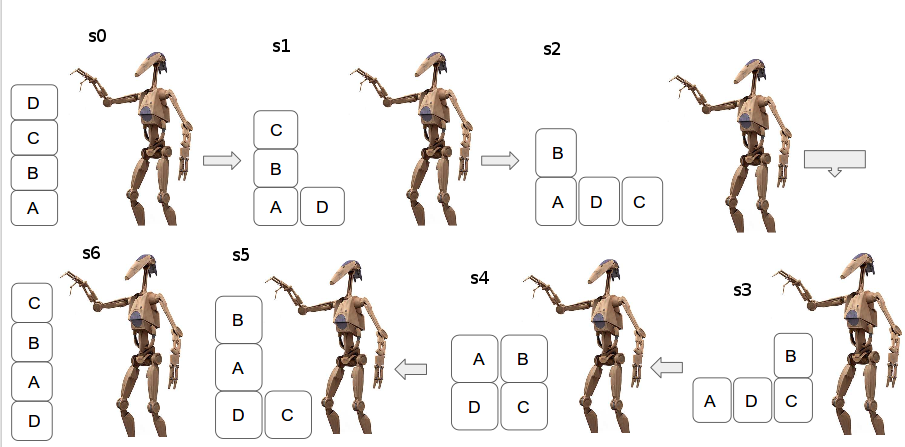
\includegraphics[scale=0.3]{StateTransitionEdit.png}
    \caption{Example of state transition, from one to another}
    \label{fig:StateTransition}
\end{figure}
In Figure \ref{fig:StateTransition} we have 7 states in total ranging from $s_0, s_1, s_2, s_3, s_4, s_5, s_6$. After an action has been performed it leads us to the next state. Now we can put the classical planning definition into some perspective, for example, we have 4 blocks, labelled A, B, C and D. A robot R1, an initial state onTable(A, B) onTable(C, D) meaning that all 4 blocks are placed on a table, and a simple goal state of on(A, B) on(C, D) meaning that we need to stack $(A\wedge B)$ and $(C\wedge D)$. This is a simplistic way of explaining the methods involved in planning and how a planner would solve this problem. What a person would do is assess the quickest and most efficient way (to them) to solve. Taking block A and putting it on top of B, and the same for block C and block D. A planner (depending on the algorithm) will create a type of search tree and explore each state by generating successors of already-explored states.
\begin{figure}[!htb]
    \centering
    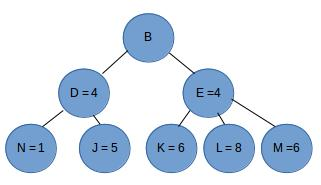
\includegraphics[scale=2.0,width=0.70\textwidth]{TreeExample.jpg}
    \caption{Basic example of a search tree with starting node B and goal node N\cite{PlanningBook}}
    \label{fig:Tree Example}
\end{figure}

As you can see in Figure \ref{fig:Tree Example}, if the goal was to find the shortest path from an initial state B to a goal state N, the planning algorithm would expand D and E, and from this would assess that N is a child of D. The algorithm would quickly find the node N in the tree graph and the cost for getting from B to N would be 5. 
\section{The Goal}
The goal for this thesis is to evaluate and test the techniques used in the PDDL4J library. In my opinion, the range of algorithms that can be used for planning is very wide and the current approaches are not optimal.  
In the following sections we will discuss the types of technologies that will be used throughout this thesis. We will start with the PDDL language in which domains and problems are encoded, then I will speak briefly about the PDDL4J library, introduce heuristics and finish with satisfiability problems.
\section{PDDL}
With the basics on planning covered, we can see how it is incorporated into the PDDL (Planning Domain Description Language), which is the main language for classical planning problems and domains. PDDL is used to express what predicates there are, what actions are possible, action structures and what the effects of those actions would be.\cite{PDDL1.2} Each type of problem for example, 'Blocksworld' or 'Mystery', will have a number of problems ranging from easy to hard, as well as a domain. The domain will provide the actions of what can be done, for example picking up a block as in Figure \ref{fig:StateTransition}. The problem file will begin with the objects that tell the planner how many items there are, such as 'objects: A B C D - blocks'; the more objects, the harder the problem. It will also define an initial state which will let the planner know what state the blocks are in, for example '(onTable B)', and will provide a goal state which the planner must satisfy. 
The main components of the PDDL represented as a planning task are:
\begin{itemize}
\item Objects = The blocks in this case (A, B, C, D)
\item Predicates = Properties of objects – these can be true or false. For example: Is A a block?  
\item  Initial state and goal state = The starting state of the world and the goal state of the world. All blocks are on the table and the goal is for them to be stacked in a specific order.
\item Operators/Actions = The actions that can be used to complete the task, broken down into preconditions and effects. Each precondition and effect can be positive or negative. \ldots
\end{itemize}
Each of the above are split between the domain file and the problem file. The domain handles the predicates and actions while the problem handles the initial state, goal state and the objects. 

If we look at the domain we can see the schema for the Blocksworld problem (see Figure \ref{fig:Blocksworld Domain} below). Inside we have some requirements at the top which tells the planner if it's able to solve the problem. It does this by informing the planner of the types of actions it will find within the domain, conditional effects, equality etc. As PDDL is a huge language, there are multiple subsets that have been created because very few planners would be able to incorporate all versions of the PDDL language. 
\begin{figure}[!htb]
    \centering
    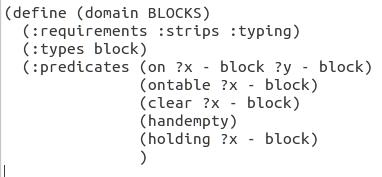
\includegraphics[scale=1.8,width=0.70\textwidth]{BlocksworldDomain1.jpg}
    \caption{Example of domain schema from Blocksworld domain}
    \label{fig:Blocksworld Domain}
\end{figure}
Next the actions associated with that domain will be specified. The actions will reflect the requirements (Figure \ref{fig:Blocksworld Pick-up Action}) and the planner will use these actions to help it solve the problem. 
\begin{figure}[h]
    \centering
    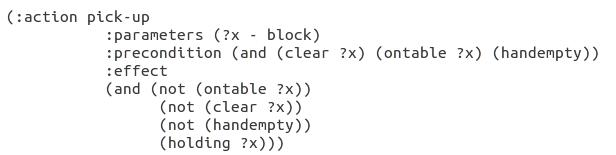
\includegraphics[scale=2.0,width=0.70\textwidth]{BlocksworldDomainAction.jpg}
    \caption{Example of an action pick-up from Blocksworld domain}
    \label{fig:Blocksworld Pick-up Action}
\end{figure}
\\
\\
The action in Figure \ref{fig:Blocksworld Pick-up Action} is a pick-up action; it tells the planner that it can only pick up one block at one time and, when it is picked up, it is at location x. An action can only be executed when the preconditions of that action are fulfilled; when the execution takes place, this generates effects, i.e. changes within the environment, for example:
\begin{itemize}
\item Block A has been picked up = Action
\item Clear A must be true before the robot can pick it up, therefore, nothing can be on top of block A = Precondition of the action PickUp
\item The negative effect of this action is that the Block A is now not on the table and the robot's hand is not empty. The positive effect of this action is that the robot is now holding Block A = Negative/Positive effects 
\end{itemize}

The planner will use actions like these, and others that are coded in a similar fashion, to complete a problem. Below is a problem example which shows the objects (in this case 4), the initial problem stating the blocks that are clear, the blocks that are on the table and that the robot's hand is empty, and then finally the goal state. 
%INPUT PROBLEM PHOTO HERE
\begin{figure}[!htb]
    \centering
    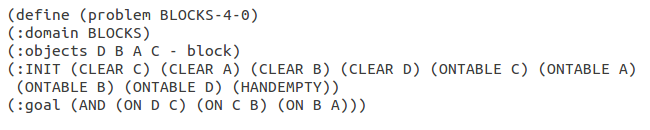
\includegraphics[scale=2.0,width=0.70\textwidth]{BlocksworldProblem.png}
    \caption{Example of a problem from Blocksworld 
    domain}
    \label{fig:Blocksworld Problem}
\end{figure}
\\
To tie all of the above together, the domain will provide the planner with the actions along with preconditions and effects for that action, and the problem will provide an initial state and a goal state that the planner must reach in order to satisfy the problem. 
\\
Now we can define a PDDL task by a 3-tuple $\Pi$ = ($S_0, G_n, O)$ where
\begin{itemize}
\item $S_0$ = Is a finite set of ground atoms called the initial state
\item $G_n$ = Is a closed formula called the goal formula
\item $O$ = Is a finite set of PDDL actions \cite{ConciseDomain} \ldots
\end{itemize} 

The initial state and goal state are the same as previously explained but, as the initial state begins at 0 and the goal state at \textit{n}, we are not sure where it is within the sequence. The axioms help us define predicates based on basic predicates. As seen by the example "given an \textit{ontop} predicate, we can define its transitive closure \textit{above} with the two axioms \textit{$above(x,y) \leftarrow ontop(x,y)$} and \textit{$above(x,z) \leftarrow \exists y(ontop(x,y)\wedge above(y,z))$}" \cite{ConciseDomain} With axioms like this, we ensure the evaluation is well defined and contains specific rules such as "ontable(A) is true when ontable(A) is actually false".   

\section{PDDL4J}

As discussed earlier, PDDL4J was created by Damien Pellier. The main components of the planner break down into three broad categories: 
\begin{itemize}
\item Preprocessing 
\item Search algorithm 
\item Heuristics
\end{itemize}
Using these three categories in unison creates a well-formed planner. The preprocessing side will take in all the facts from the domain of a PDDL problem and change each action condition using the variables, such as Block A, Block B etc. 
\begin{verbatim}
(:action pick-up
		:parameters (A - block) 
		:precondition (and (clear B)(ontable B)(handempty))
		:effect
		(and(not(ontable A)) 
\end{verbatim}
In each problem, the objects are known from the beginning, so the preprocessing side of the planner will instantiate each operator with all possibilities. As well as, this there are a number of steps that need to taken into account before the final representation is presented to the search algorithm and heuristic. When the domain and problem are encoded, logical simplification is performed to convert the problem to a bitset representation as the final outcome.
%Check new paragraph was inserted
\\
\\
There are a number of different planning algorithms that can be used to find a solution to a problem; the PDDL4J library uses an algorithm called A*. The main idea behind A* is that it searches through all possible paths to the goal to find the shortest path. It is an iterative algorithm and, after each iteration, it decides which of the nodes to expand of the partial plan it has already made until it reaches the goal and computes the fastest route. It does this by using the simple function
\textit{f(n)= g(n) + h(n)} \cite{MinimumCostPaths} where
\begin{itemize}
\item\textit{n} = the last node in the path
\item\textit{g(n)} = the cost of the path from the start to \textit{n}
\item\textit{h(n)} = the heuristic that estimates the cost from \textit{n} to the goal
\end{itemize}

The A* algorithm will use the function above and then try to find the best and less costly route. It does this by examining the vertex $n$ that has the lowest $f(n)$ score. For example, if the cost from getting from a starting node \textit{A} to a goal node \textit{D} had two routes, one giving a total cost of 4 and another 6, A* will always choose the route with minimal cost. But A* cannot work on its own to find a solution to a problem, it needs to use a heuristic to assist it and guide it to the goal.

The role of a heuristic is to help look for an answer to a particular problem. It does not tell the algorithm what to find but only how to look for a potential solution. Within the PDDL4J library and with the A* algorithm, each heuristic plays a different role when used to help find a solution but will provide the same basic level of help, which is estimating the distance to the goal. 
\\
\\
In the context of mathematics, the Manhattan distance is the distance between two points measured along axes at right angles\cite{ManhattanDistance}. It can be written as $|x_1 - x_2| + |y_1 - y_2|$ when we have two points $p_1$ at $(x_1, y_1)$ and $p_2$ at $(x_2, y_2)$. This type of function can be used with the A* algorithm in the form of a heuristic to find the shortest path from $p_1$ to $p_2$. If we translate that into a heuristic function in the Java programming language, it will look more like this:
\begin{verbatim}
int distance = Math.abs(x1 - x2) + Math.abs(y1 - y2);
\end{verbatim}

If we wanted to incorporate the function above with A*, we would create a small algorithm that would increase the value of \textit{g} by \textit{distance} and decrease \textit{h} by \textit{distance} as we move closer to the goal. So, regarding, the A* function \textit{f(n)}, the A* function should have the same value as the \textit{distance} function defined above. If the two match then we would say that this heuristic is "admissible". 

Within the world of heuristics, two definitions exist: "admissible" and "non admissible". What is an admissible heuristic? We can say a heuristic \textit{h} is admissible if $h(s) \leq h^*(s)$ for all states \textit{s}. In other words, when estimating the distance from a starting node to a goal node, it does not overestimate. Then for a non admissible heuristic, there is a possibility that it will overestimate or underestimate the distance. Within the PDDL4J library there are two admissible heuristics, $h^m$ and $h^{MAX}$, but these will be discussed later. 

\section{Satisfiability Problem}
In the previous subsections, we looked at PDDL and how it works. This section and one in Chapter \ref{Chapter2} dedicated to a set of problems termed satisfiability (SAT) problems. These are a set of expressions which are boolean, which means there are only two possible outcomes, i.e. either true or false. It is expressed in propositional logic and uses the operators AND(conjunction, $\wedge$), OR(disjunction, $\vee$) and NOT(negation, $\neg$). We say a problem is satisfiable if all the variables can be set to true or false. There is a particular structure that needs to be kept when working with satisfiability problems – we will look at the notation briefly. 
\begin{itemize}
\item A literal can be positive or negative – $p_1$ is positive and $\neg p_2$ is negative. 
\item A clause is a disjunction of literals.
\item A formula is in conjunctive normal form (CNF) if it is a conjunction of clauses.\cite{SurverySat}
\end{itemize}
As stated above, we have $p_1$ and $\neg p_2$. $p_1\vee \neg p_2$ is a clause and $(p_1\vee \neg p_2) \wedge (\neg p_1 \vee p_2 \wedge p_3) \wedge \neg p_1$ is a formula in conjunctive normal form. 
If we set $p_1$ = false, $p_2$ = false we get $(F \vee T) \wedge(T \vee F \vee p_3) \wedge T$ 
\\
($p_3$ is arbitrary which means it is not assigned a value)
\\
\\
Using CNF rules\cite{Conjunctive}, we can deduce the above formula as $T \wedge T \wedge T$ = True.
As this formula has been classed as true because of the rules applied in propositional logic, we begin to see how it can be useful in terms of planners and solving complex problems.